\documentclass[12pt]{article}
\usepackage{graphicx}
\usepackage{natbib}
\usepackage{amssymb}
\usepackage{amsmath}
\usepackage{caption}
\usepackage{subcaption}
\usepackage{longtable}
\usepackage{rotating}
\usepackage{float}
\oddsidemargin 0pt
\textwidth 6.5in
\topmargin -0.65in
\textheight 9.25in

\begin{document}
\begin{center}
\textbf{Elements of Fun: Predicting the Ratings and Prices of Board Games}

Andrew Riddle
\end{center}

\section{Motivation}
What makes a board game fun to play? Perhaps it depends on the number of players that can play the game or the complexity of the game, or some other factors. If you could predict how well certain games wil do based on certain intrinsic characteristics of the game, measured by a numerical rating from many people, you could use that information to predict how well a new game will sell or how good an older game is that has no or very little review data available. Using sale price from historical sales as the target instead of game rating would allow for a pricing tool for new games going to market. With that, you could also identify segments of the board game market that lead to the highest priced games and focus on developing those types of games at a cheaper production cost to maximize profit.

\section{Data Acquisition}
The game data were taken from boardgamegeek.com, using their object API located at https://www.boardgamegeek.com/xmlapi2/thing. All games with a game ID between 1 and 110,317 were queried. About half of these (49,173) were board games, specified by the object type. In addition to the basic game features, the API can also return some statistics about the game based on user reviews as well as sale listings on their website (by users). The statistics include the average user rating on a scale from 1 to 10 as well as a bayesian average of the user rating (the "geek rating"), which the website uses to rank their games. If there are no user reviews, the game gets a geek rating of 0 and has no rank. Since the original goal was to use the geek rating as the target variable for a metric of the quality of a game, only games that have a defined rating (i.e. games that have user reviews) can be used. Of the ~50,000 games that I had data for, only 10,000 had ratings. 8,000 of these games hade available market data and it was this final subset of games that was used in the analysis. Table 1 shows a list of the column data returned by the API as well as a brief description of each column. 

\begin{table}[ht]{\small \textbf{Table 1}. Columns.} \\
\centering
\begin{tabular*}{\textwidth}{llc}
\hline\hline
Column Name & Description & Data Type\\
\hline
age & Minimum suggested age for players & int \\
avg\_rating & Average user rating (1-10) & float \\
avg\_time & Average length of a game (min) & float \\
category & Category or genre the game belongs to & str \\
designer & Designer(s) of the game & str \\
game\_id & ID used to identify the game & int \\
geek\_rating & Bayesian average of the user ratings; used to rank games & float \\
market & Sales listings by users of the site & dict \\
max\_players & Maximum number of players the game can support & int \\
max\_time & Maximum time a game takes (min) & int \\
mechanic & Mechanic(s) by which the game progresses & str \\
min\_players & Minimum number of players required to play & int \\
min\_time & Minimum time required to play a game (min) & int \\
name & Name of the game & str \\
num\_votes & Number of user ratings & int \\
numcomments & Number of comments left by users & int \\
numweights & Number of user reviews for the game weight (complexity) & int \\
owned & Number of users thay own the game & int \\
rank & Game rank & int \\
trading & Number of users trading the game & int \\
wanting & Number of users actively seeking the game & int \\
wishing & Number of users wishing for the game & int \\
weight & Average weight (complexity) rating left by users (1-5) & float \\
year & Year the game was released & int \\
\hline
\end{tabular*}
\end{table}

\section{Preprocessing}
The first step was to parse the market data into a usable form; the data coming out of the API consist of individual sale listings for each game by users, including the date, price, condition, and currency. I used historical exchange rates pulled from the API at https://api.fixer.io in conjuction with the year of the listing to convert each sale to USD. No adjustment was made for inflation. Once all prices were converted to USD, the median price was used as the feature for that game. The median price was used as it's less susceptible to outliers than the mean. There were a handful of games with very high prices ($>$ \$500), so i did 2 rounds of sigma clipping, setting values higher than 3 times the standard deviation from the mean equal to 3 times the standard deviation plus the mean each time. This reduced the maximum price from \$10,000 to \$200, with a distribution pictured in Fig. 1. This was done for two reasons: the first being that linear models don't handle outliers well, and the second being that the prices on some of these games might not be reliable or they might be for a special edition of the game that doesn't reflect the price of the standard version.

\begin{figure}[ht]
\centering
\begin{minipage}{.48\textwidth}
\centering
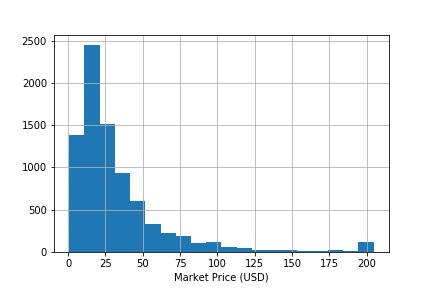
\includegraphics[height=6cm]{market_price_hist.png}
\end{minipage} \hfil
\centering
\begin{minipage}{.48\textwidth}
\centering
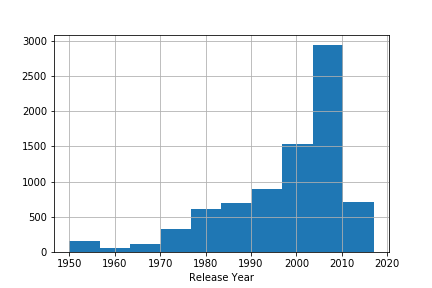
\includegraphics[height=6cm]{market_year_hist.png}
\end{minipage}
\caption{\small $Left$: Histogram of the available market data. $Right$: Histogram of release year after imputing very old games to 1950.}
\end{figure}

There were four other features with outliers: year, max\_players, avg\_time, and age. The year column had a massive range as the list of games includes very old game like Go and Backgammon (both "released" over 2000 years ago). To accomodate for this I set a minimum year value of 1950, imputing any values less than that to be 1950. I also created a "Classic" feature that equals 1 for games released before 1900 and 0 for games released after. A similar process was done for the other three columns. For max\_players a maximum cutoff of 20 was set as there are very few games beyong this point and the difference between 20 players and 20+ players isn't that significant. For the avg\_time a maximum cutoff of 480 minutes was used. I used 21 as the uper bound on age as a minimum suggested age beyond that doesn't make sense in terms of maturity/things you are legaly allowed to do (e.g purchase alcohol). There are also some games that have no user reviews on the weight (complexity) of the game and thus have a value of 0 in that column. I imputed this missing data using the median weight of all games for which there was a non-zero weight.

Keeping in mind that the goal of the project is to to able to predict the game rating, which is a proxy of the popularity, of games that are brand new or have no user reviews, any feature tied to user data must be thrown out. For this reason, I droped avg\_rating, num\_votes, numcomments, numweights, owned, trading, wanting, and wishing. I created a column called name\_len that is the number of characters in the game name under the theory that shorter names might be catchier and thus more popular. Once these step were taken, I used a a heatmap to check for colinear features and to get an idea of which features might have the most predictive power (see Fig. 2). The features related to time spent playing the game are all colinear (Pearson correlation coefficient $>$ 0.8). I chose to keep just the avg\_time of those three features. A Seaborn pairplot of the remaining numerical columns is shown in Figure 3. The game ID was left in temporarily so that the results can be matched up after the analysis, but will be removed before being fed into any mdoels.

\begin{figure}[ht]
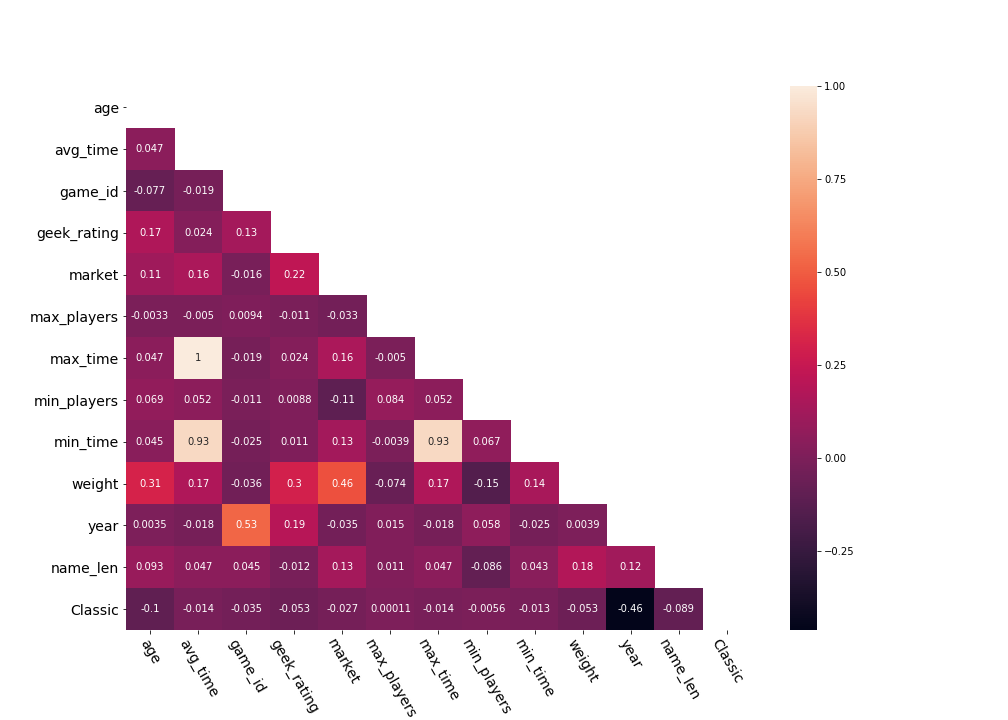
\includegraphics[width=20cm]{ranked_df_heatmap.png}
\caption{\small Heatmap of numerical columns showing the Pearson correlation coefficient.}
\end{figure}

\begin{figure}[ht]
\centering
\resizebox{\linewidth}{!}{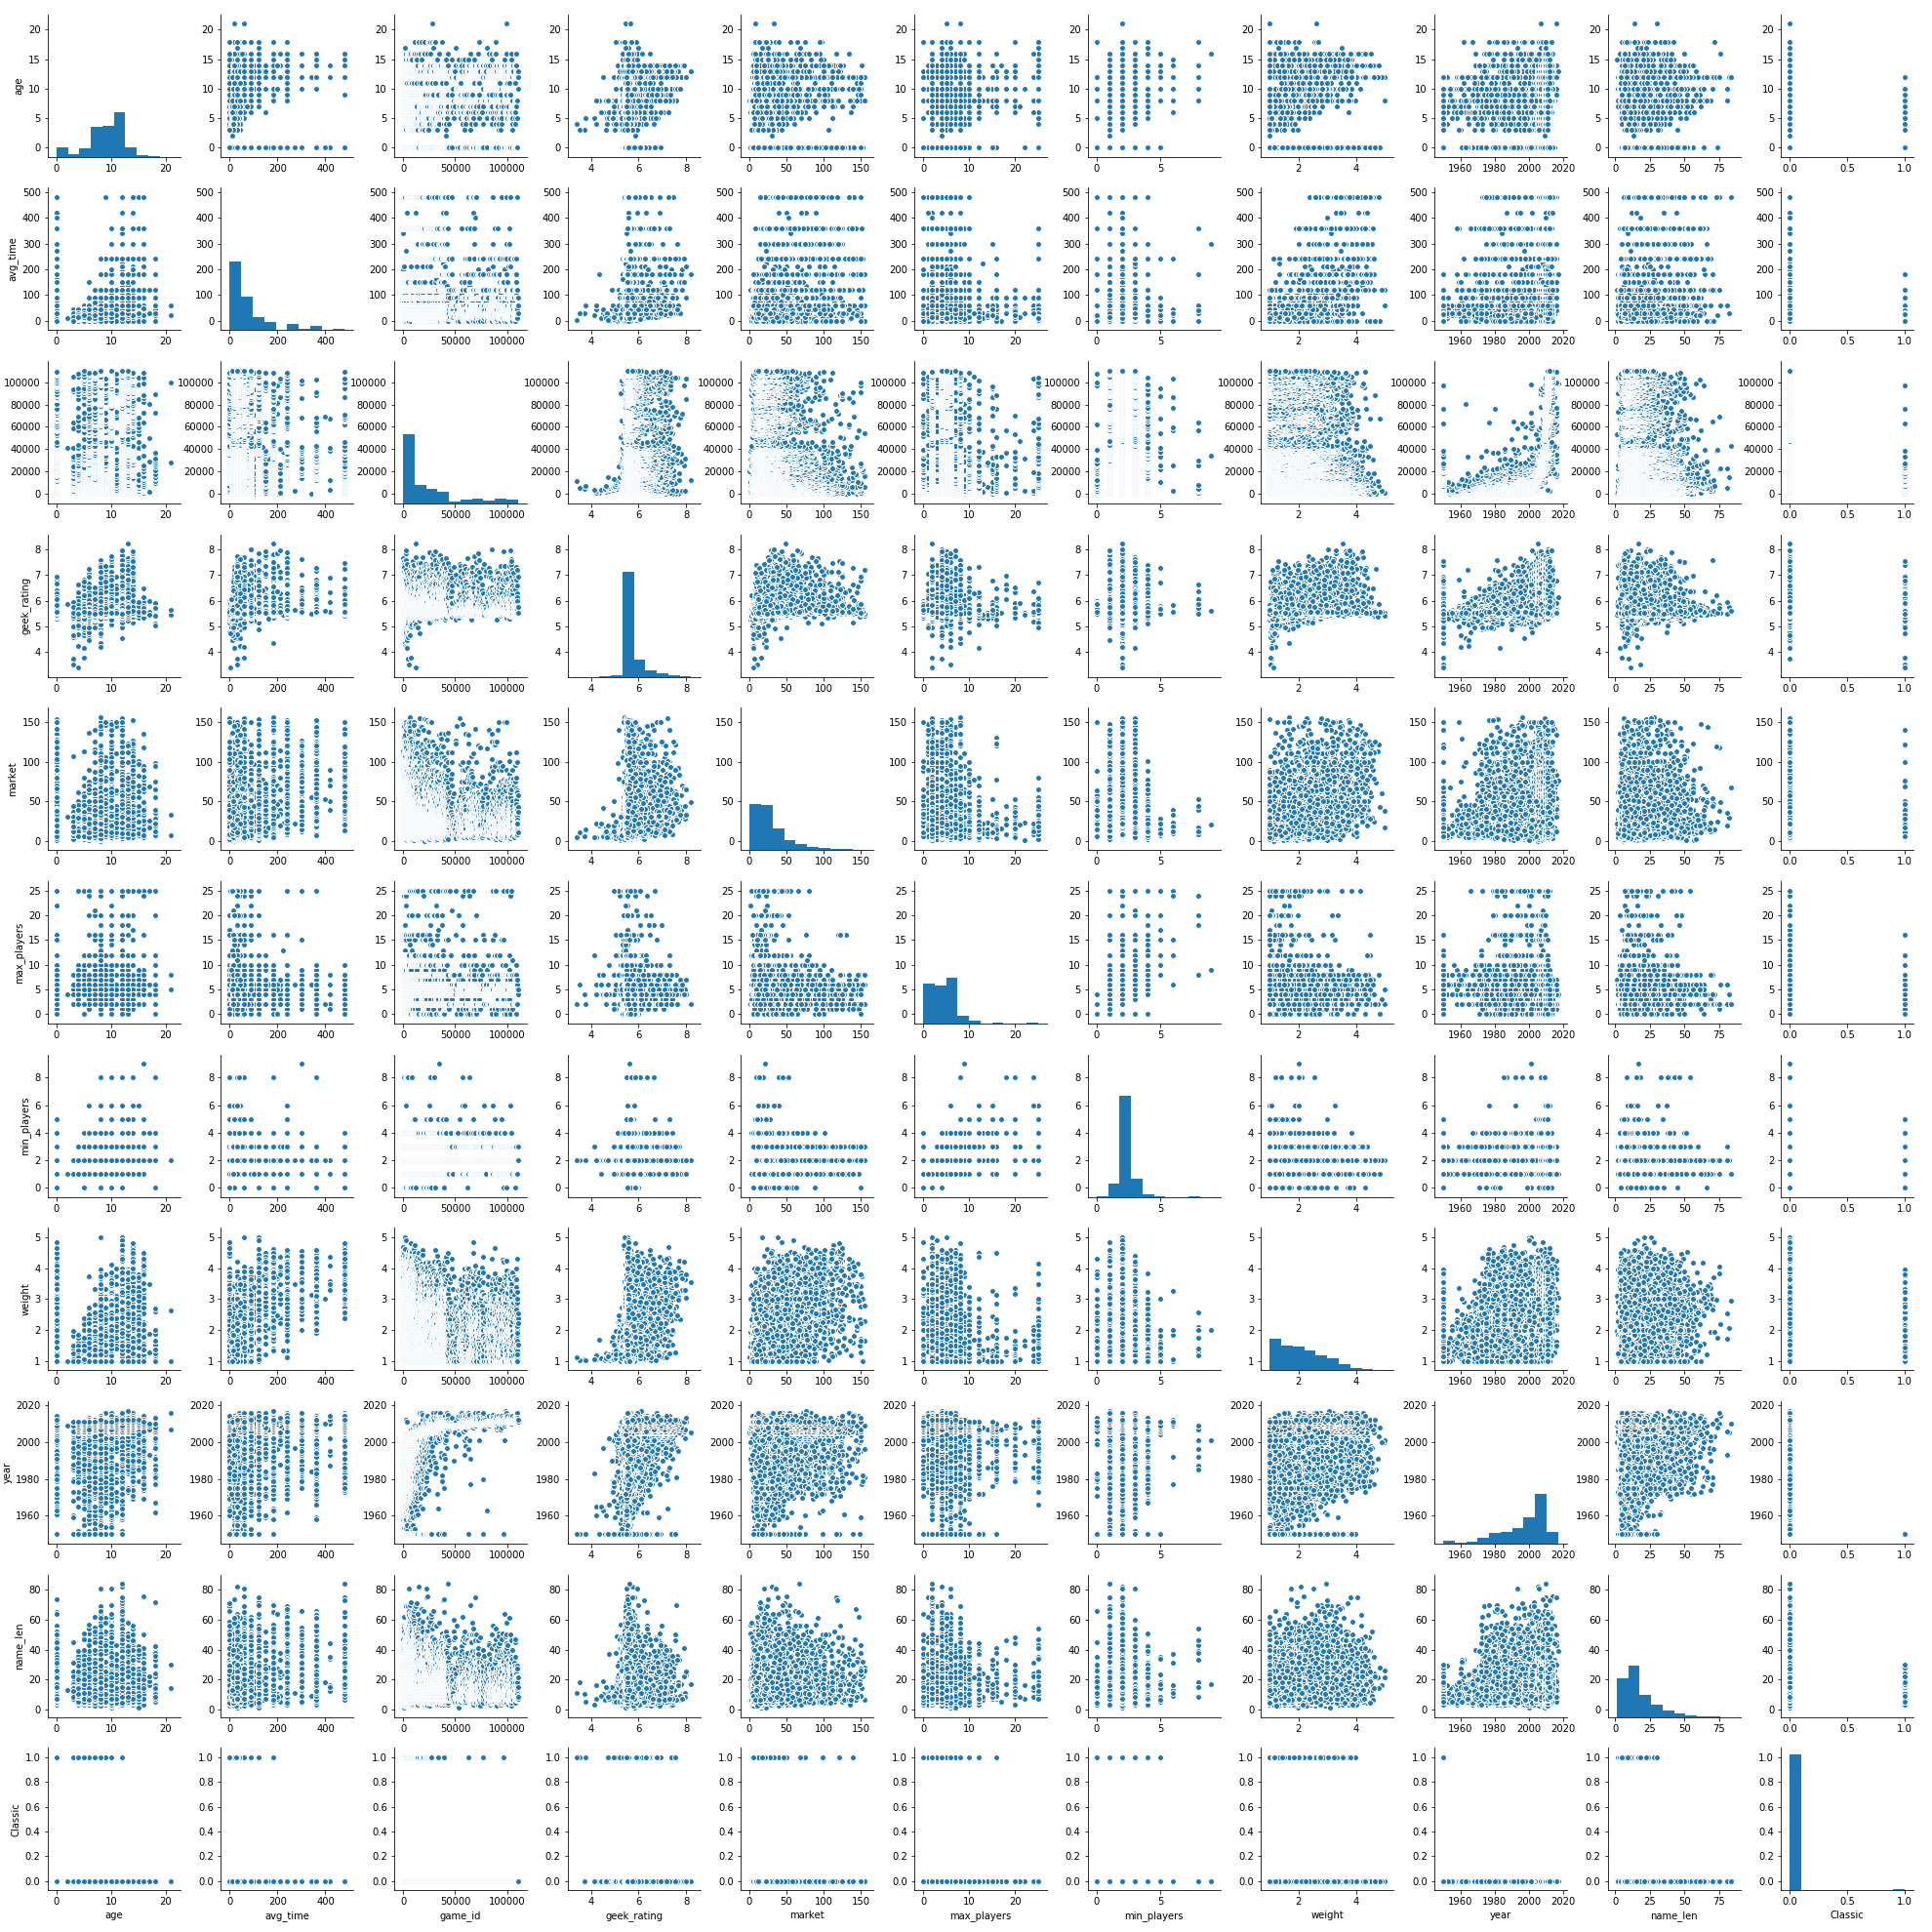
\includegraphics{pairplot.png}}
\caption{\small Seaborn pairplot of numerical columns.}
\end{figure}

That leaves the four text fields to be dealt with: name, mechanic, category, and designer. Other than the name\_len, no other features were engineered from the name column as the names are too specific to each game. For the other three I used a CountVecotorizer to convert the text data into numerical columns. Each game can have multiple entries in a column (it can have multiple mechanic types, categories, and designers), but each entry is only ever listed once (per game).  The vectorizer turns each column into a distinct bag of words and then creates a column for each word that is a 1 if the game has that mechanic, category, or designer and 0 otherwise. Before the count vectorizer is used, missing data in each text field is changed to be ``Designer Unknown'' for the designer column and so forth. For the designer column, I used a minimum document frequency of 7. In other words, a designer had to be listed on 7 games before he or she was added to the bag of words for that column. This was done so that only designers with some pedigree would be included. A few different numbers were tried for this minimum document frequency, but 7 was found to produce the best results.

Each of the numeric columns (not counting the vectorized text columns) was passed through a sigma clipping function that changed values greater than 3 standard deviations from the mean to be at the edge of that boundary. Finally, they were passed through a MinMax scaler so that each column would be in the range from 0 to 1. This is done so that each feature starts with an equal weight in the models, although it's not necessary for tree-based models. As there are many features after using the count vectorizer, I thought using SVD might be helpful. However, when looking at the explained variance with each component (c.f. Fig. 4) there is no ``elbow'', and thus I decided to not use SVD so as to preserve feature importances/weights in the models.

\begin{figure}[ht]
\centering
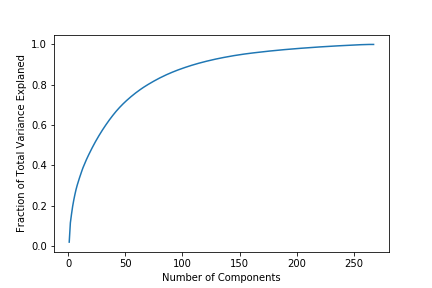
\includegraphics[width=10cm]{market_svd.png}
\caption{\small Cumulative explained variance ratio as you add more SVD components.}
\end{figure}

\section{Modeling}
I built the steps discussed in \S3 into a pipeline for analysis. The full data set was split into 80-20 train/test partitions twice. The first split was to generate a holdout data set to use for final testing, while the second split was done for the traditional validation purposes. This means that the models were trained on 64\% of the total data set with 16\% used as validation data and 20\% used as holdout data.

A number of different regression models were tested on the training data and validated on the test set, including Random Forest, Elastic Net, Gradient Boosted Tree, K-Neighbors, SVM, and a Neural Network. For each model I did a grid search over relevant hyperparameters. The parameter grid I tried for each model is shown in Table 2.

\begin{table}[ht]{\small \textbf{Table 2}. Model Parameter Grids} \\
\centering
\begin{tabular*}{.7\textwidth}{lc}
\hline\hline
\multicolumn{2}{c}{Random Forest (RF)} \\
\hline
Parameter & Grid \\
\hline
min\_samples\_leaf & 1, 3, 5, 7 \\
n\_estimators & 25, 50, 75, 100, 125, 150 \\
max\_features & None, 1/3  \\
\hline
\multicolumn{2}{c}{} \\
\multicolumn{2}{c}{Elastic Net (EN)} \\
\hline
Parameter & Grid \\
\hline
$\alpha$ & 0.001, 0.01, 0.1, 1, 10 \\
l1\_ratio & 0.01, 0.05, 0.1, 0.25, 0.5, 0.8, 0.9 \\
fit\_intercept & True, False \\
\hline
\multicolumn{2}{c}{} \\
\multicolumn{2}{c}{Gradient Boosted Tree (GBT)} \\
\hline
Parameter & Grid \\
\hline
learning rate & 0.05, 0.1, 0.3 \\
max\_depth & 3, 5, 7, 9 \\
max\_features & None, 1/3 \\
n\_estimators & 100,150,200 \\
subsample & 0.5, 0.8, 1 \\
\hline
\multicolumn{2}{c}{} \\
\multicolumn{2}{c}{K-Nearest Neighbors (KNN)} \\
\hline
Parameter & Grid \\
\hline
n\_neighbors & 3-21 \\
\hline
\multicolumn{2}{c}{} \\
\multicolumn{2}{c}{Support Vector Machine (SVM)} \\
\hline
Parameter & Grid \\
\hline
kernel & rbf, linear, poly \\
degree & 2, 3, 4 \\
$\gamma$ & auto, 0.1, 1, 10 \\
C & 0.1, 1, 10 \\
$\epsilon$ & 0.05, 0.1, 0.2, 0.4 \\
\hline
\multicolumn{2}{c}{} \\
\multicolumn{2}{c}{Neural Network} \\
\hline
Parameter & Grid \\
\hline
Dropout & 0, 0.25, 0.5 \\
Nodes in 1st hidden layer & 25, 50, 75, 100, 150 \\
Nodes in 2nd hidden layer & 0, 25, 50 \\
\hline
\end{tabular*}
\end{table}


\section{Results}


\section{Future Plans}


\end{document}